\chapter{Phase 3}


\section{Algorithm Selection}


\subsection{Justification for choosing Gradient Boosting}

In phase 2 of this project, six machine learning algorithms were evaluated: K-Nearest Neighbors (KNN), Naive Bayes, Logistic Regression, Support Vector Machines (SVM), Decision Trees, and Gradient Boosting. Each algorithm underwent tuning and assessment to determine its effectiveness in predicting anemia levels.

KNN was optimized using grid search with cross-validation, achieving an accuracy of 61.86\%. While it showed reasonable performance, struggles were evident in predicting less represented anemia levels, particularly 0 and 4. Naive Bayes, despite its simple assumption of feature independence, demonstrated effectiveness with an accuracy of 65.99\%, particularly excelling in predicting level 0.

Logistic Regression, with hyperparameter tuning via grid search, achieved an accuracy of 86.58\%. While showing strong performance for most anemia levels, it encountered difficulty in predicting level 0. SVM, utilizing randomized search, achieved an accuracy of 88.64\%, showcasing good performance overall but facing challenges in predicting level 0.

Decision Trees and Gradient Boosting emerged as top performers. Decision Trees, after hyperparameter tuning, achieved an accuracy of 92.33\%, demonstrating high precision, recall, and F1 scores for all anemia levels, including level 0. Gradient Boosting, with randomized search, achieved an accuracy of 93.56\%, showing excellent performance across all levels, including level 0.

In conclusion, Gradient Boosting proved to be the most effective algorithm for predicting anemia levels in our dataset. Its ability to capture complex relationships between features and anemia levels, as well as their performance across all classes, highlights its suitability for this task. Hence we will be using the gradient-boosting algorithm for our final analysis

\section{Input Feature Selection}
In this phase, our analysis has pinpointed a set of 16 features that hold the utmost importance and relevance for our predictive modeling endeavors. These features have been meticulously selected based on their profound impact and contribution to the predictive accuracy of our model. Here are the features we will be considering for prediction:
\begin{itemize}
    \item Age: Age group of the mother (ranges from 1 to 80)
    \item Past Births: Number of past births of the mother (ranges from 0 to 10)
    \item First Birth Age: Age at which the mother had their first birth (ranges from 15 to 50)
    \item Hemoglobin Level: Hemoglobin level (ranges from 10 to 300)
    \item Adjusted Hemoglobin Level due to Smoking: Adjusted hemoglobin level considering smoking habits (ranges from 10 to 300)
    \item Residence Type : Whether the child resides in a rural area or urban area or unknown.
    \item Wealth Level: Wealth status of the child (Poorest, Poorer, Middle, Richer, Richest)
    \item Net Available: Availability of a mosquito net for sleeping (Yes or No)
    \item Smoke: Smoking status of the mother (Yes or No)
    \item Education Level: Education level of the mother (No, Primary, Secondary, Higher)
    \item Marital Status: Marital status of the mother (Never, Living, Married, Divorced, Separated, Widowed)
    \item Partner Co-Living: Whether the mother is co-living with a partner (Elsewhere, Unknown, Yes)
    \item Fever History: History of fever (No, Yes, Unknown)
    \item Iron Pill Taken: Whether the individual takes iron pills (No, Yes, Unknown)
    \item Family: Whether the child has a family (Yes or No)
\end{itemize}
\section{Application Building}
We employed Streamlit, a Python library, to construct the application interface. This framework simplifies the creation of interactive web applications directly from Python scripts. By leveraging Streamlit, users can effortlessly input their data about the factors influencing anemia levels, as outlined earlier. These factors encompass a range of demographic, health, and lifestyle variables. Once the user submits this input, the application employs machine learning algorithms to process the data and generate predictions regarding the individual's anemia level. This user-friendly approach enhances accessibility and enables individuals to gain insights into their health status quickly and conveniently.


\newpage
\section{Screenshots of the application}

\subsection{Input Page:}
    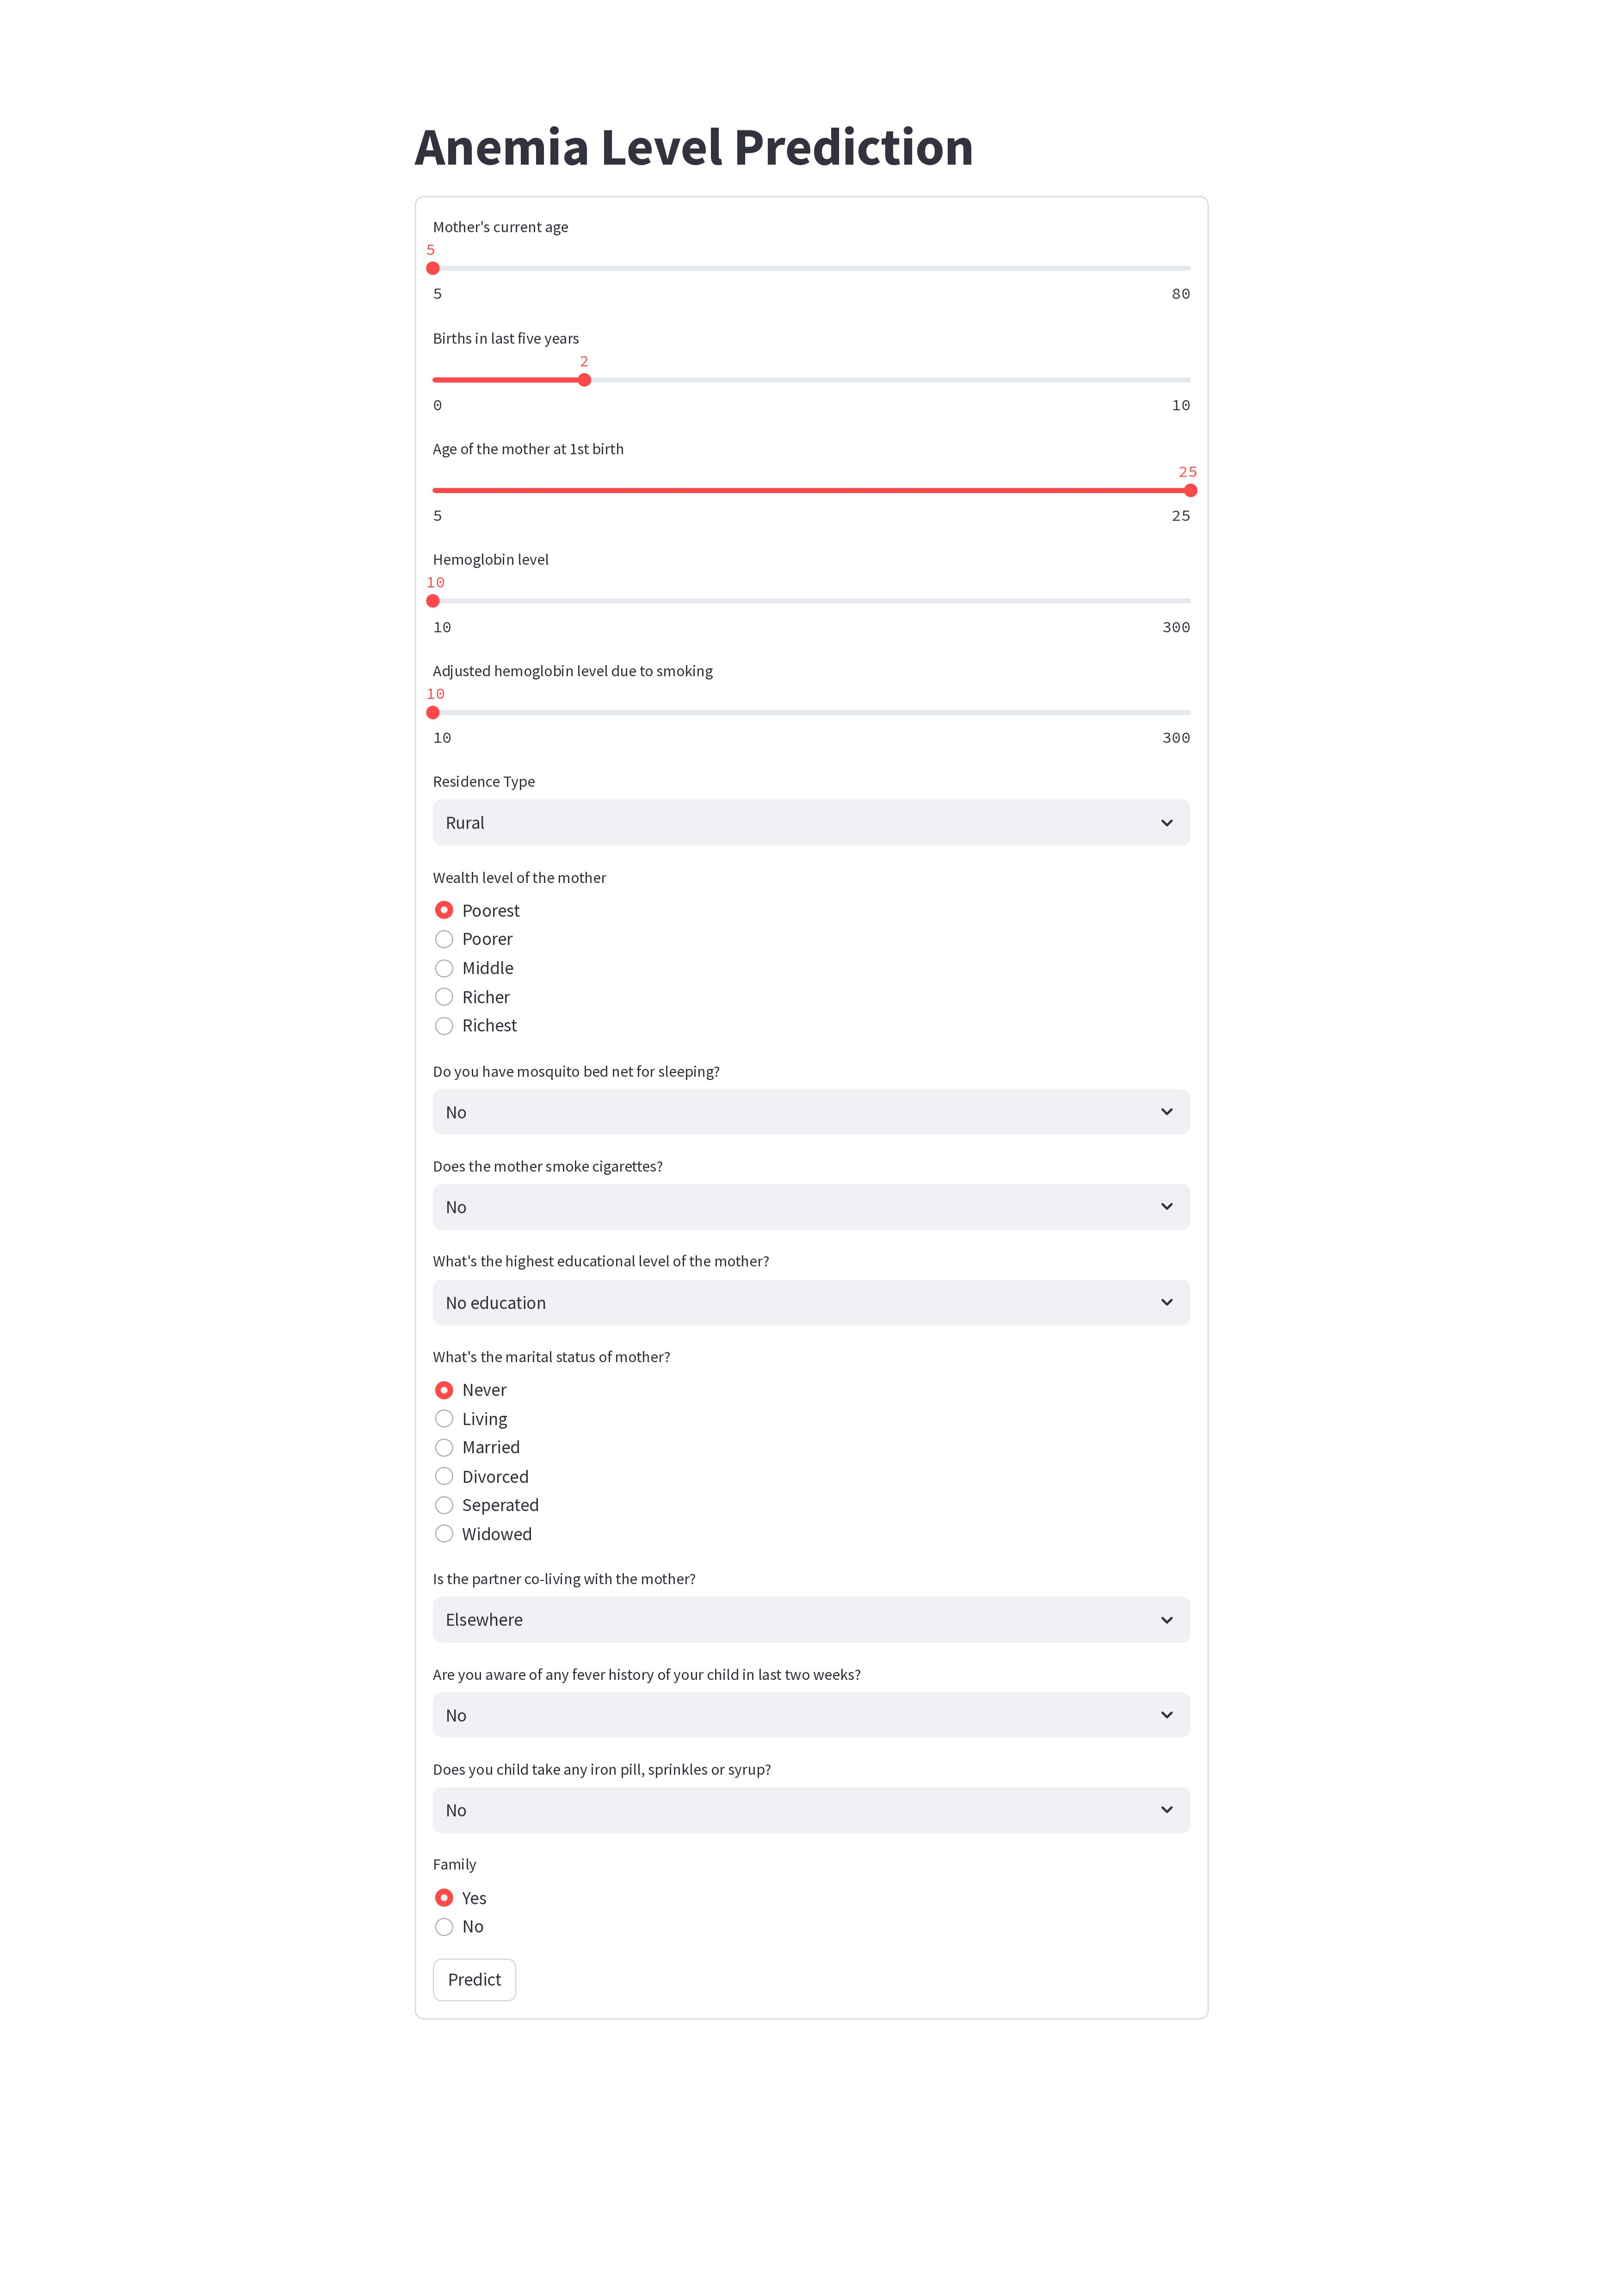
\includegraphics[width=0.75\textwidth]{input.jpg}

\newpage
\subsection{Output Page:}
    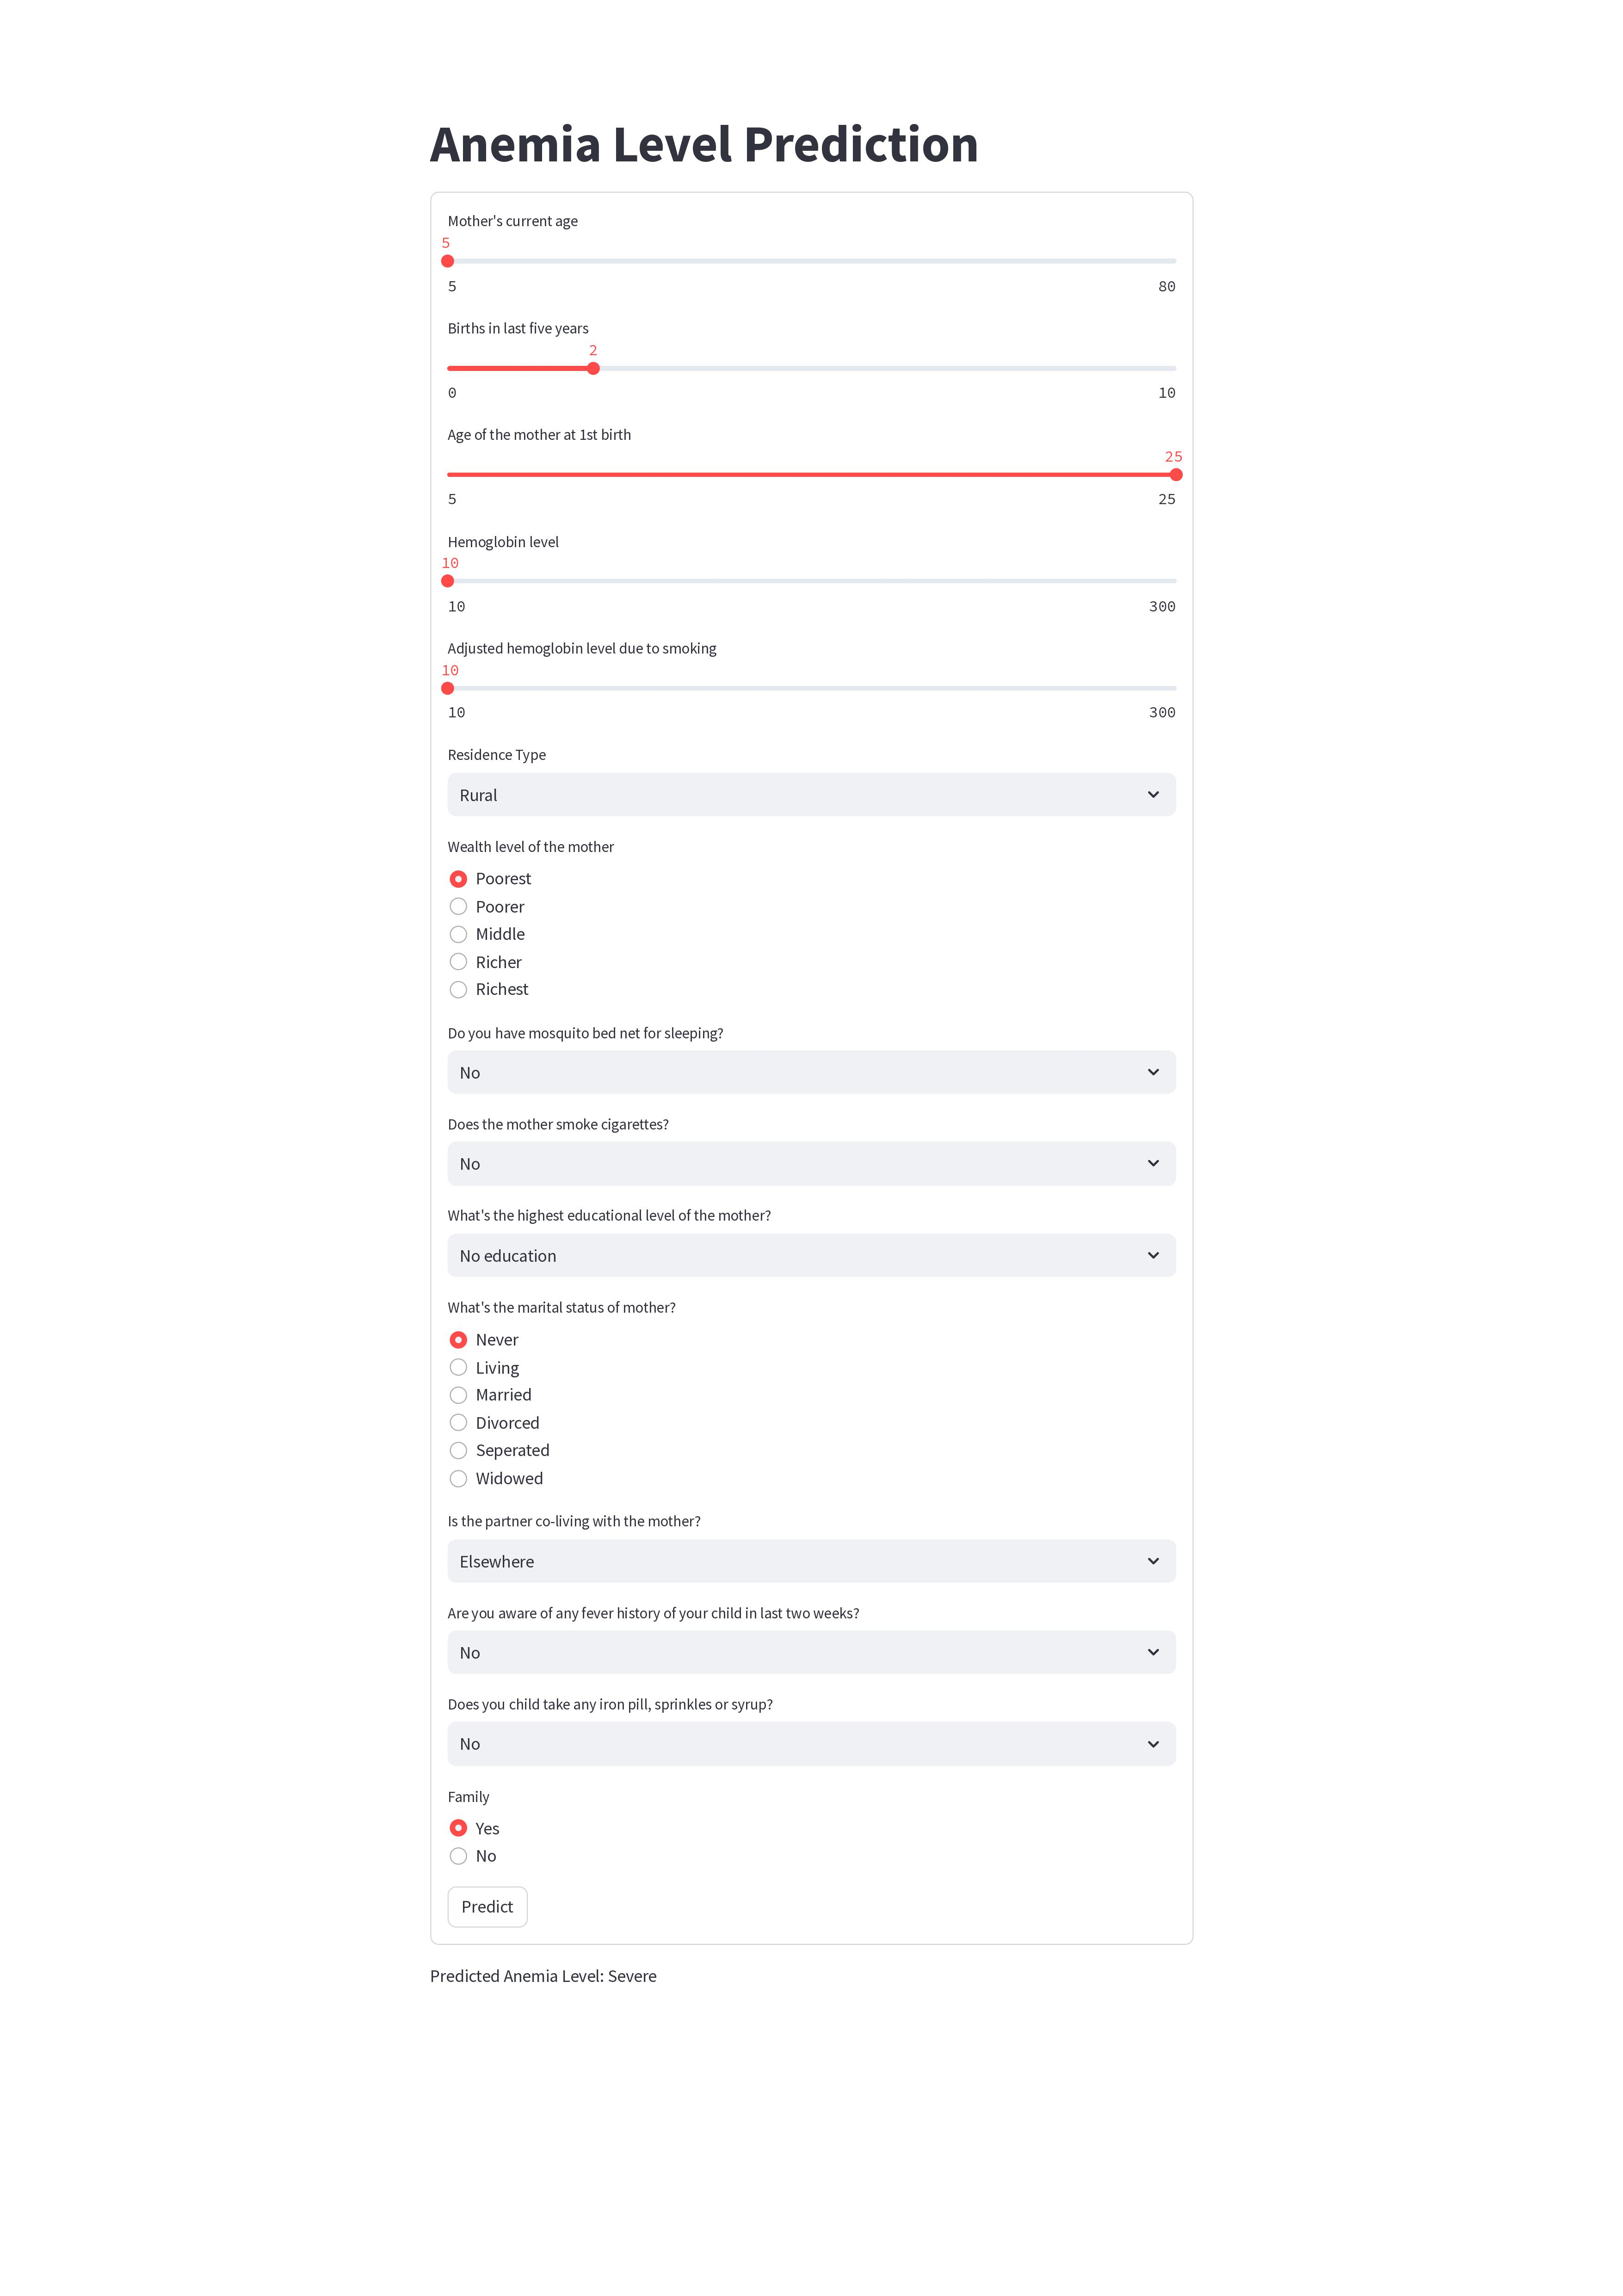
\includegraphics[width=0.75\textwidth]{output.jpg}
